\documentclass[tikz, border=2pt]{standalone}
\usepackage{amsmath}

\begin{document}
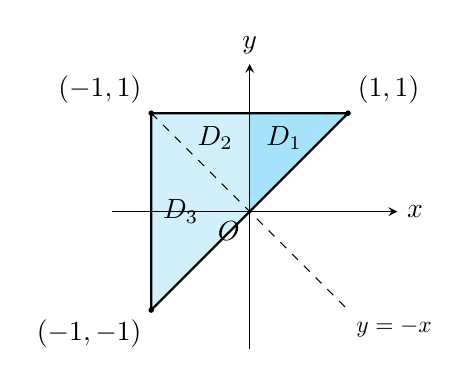
\begin{tikzpicture}[scale=1.25, >=stealth]
  \fill[cyan!18] (-1,-1) -- (-1,1) -- (1,1) -- cycle;
  \fill[cyan!35] (0,0) -- (0,1) -- (1,1) -- cycle;

  \draw[->] (-1.4,0) -- (1.5,0) node[right] {$x$};
  \draw[->] (0,-1.4) -- (0,1.5) node[above] {$y$};

  \draw[thick] (-1,-1) -- (-1,1) -- (1,1) -- cycle;
  \draw[dashed] (-1,1) -- (1,-1) node[below right, scale=0.85] {$y=-x$};

  \fill (-1,-1) circle (0.8pt) node[below left] {$(-1,-1)$};
  \fill (-1,1) circle (0.8pt) node[above left] {$(-1,1)$};
  \fill (1,1) circle (0.8pt) node[above right] {$(1,1)$};
  \node[below left] at (0,0) {$O$};

  \node at (-0.35,0.75) {$D_2$};
  \node at (-0.7,0) {$D_3$};
  \node at (0.35,0.75) {$D_1$};
\end{tikzpicture}
\end{document}
